\documentclass{lab_sheet}
\usepackage[flushleft]{threeparttable}
\usepackage[hidelinks]{hyperref}

\newcommand{\syntax}[2]{
    \lstinputlisting[label={lst:#1},caption={Syntax for #2}, captionpos=b]{./Outputs/#1.txt}
}

\newcommand{\setting}[2]{
    \begin{tabular}{C{3cm}C{5cm}C{5cm}}
        \toprule
          #1 & IP address & Subnet mask\\
          \midrule
          #2
          \bottomrule
       \end{tabular}
}
\newcommand{\customcaption}[2]{
    \begin{mdframed}[backgroundcolor=bg,innerbottommargin=-2.5em]
        \lstinputlisting[label={lst:#1},captionpos=b,style=DOS,caption={#2}]{./Outputs/#1.txt}
          \end{mdframed}
}

\newcommand{\pingtest}[1]{
    \cmdop{#1-a}{ping test from PC0 to PC1}
    \cmdop{#1-b}{ping test from PC0 to PC2}
    \cmdop{#1-c}{ping test from PC0 to PC3}
    \cmdop{#1-d}{ping test from PC1 to PC2}
    \cmdop{#1-e}{ping test from PC1 to PC3}
    \cmdop{#1-f}{ping test from PC2 to PC3}
}

\begin{document}
    \titlePage{VLAN Configuration, Forwarding Packets within VLAN and Routing Packets Between VLANs}{December 11, 2020}
    \pagenumbering{gobble}
    \tableofcontents
    \pagebreak
    \listoffigures
    \pagebreak
    \listoftables
    \pagebreak
    \lstlistoflistings
    \pagebreak
    \pagenumbering{arabic}
    \section{Objectives}
    \begin{itemize}
        \item Familiarization with VLAN and its use.
        \item To create VLANs and deliver packets between computers that are within the same VLAN.
        \item To route packets between computers at different VLANs.
    \end{itemize}
    \section{Required Tools}
\subsection{Cisco Packet Tracer}
Cisco Packet Tracer is a visual simulation software developed and distributed by Cisco Systems. Packet Tracer is a cross platform tool that allows simulated environment for modern computer network and network topologies.
\section{Simulation Activities}
\begin{figure}[H]
	\centering
	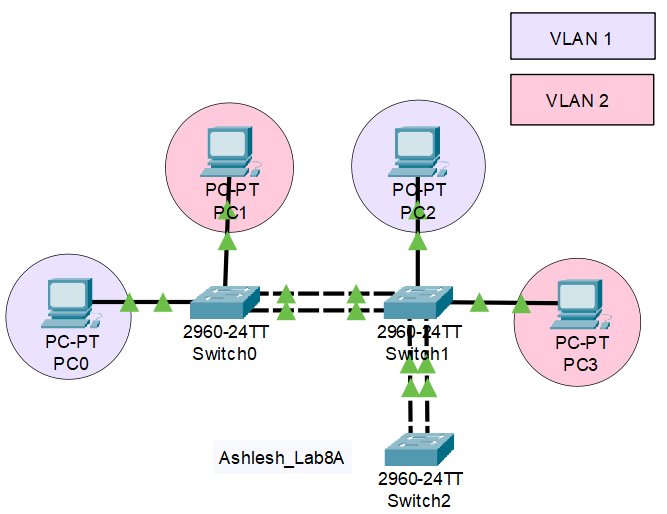
\includegraphics[scale=.9]{Figures/activitya.png}
	\caption{Simulated network for Activity A}
	\label{fig:activitya}
\end{figure}

\begin{figure}[H]
	\centering
	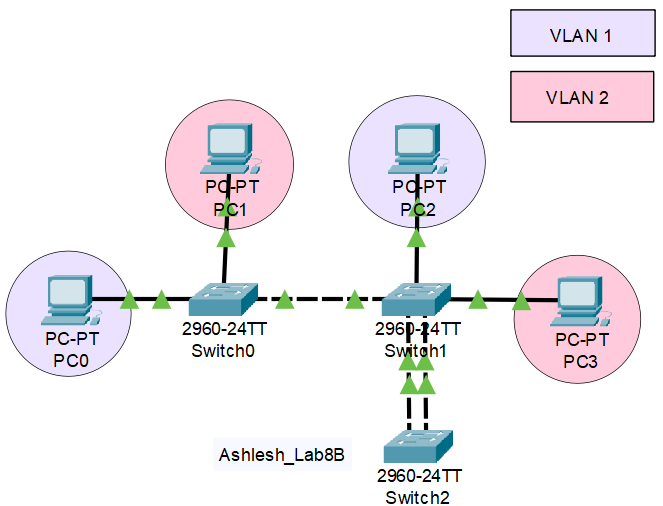
\includegraphics[scale=.9]{Figures/activityb.png}
	\caption{Simulated network for Activity B}
	\label{fig:activityb}
\end{figure}

\begin{figure}[H]
	\centering
	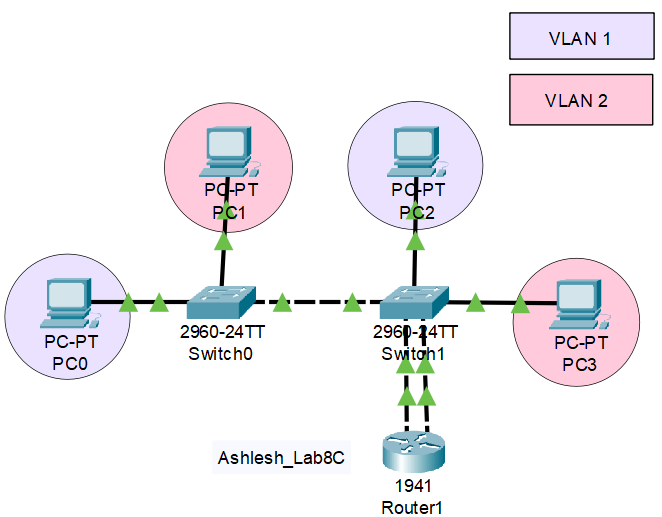
\includegraphics[scale=.9]{Figures/activityc.png}
	\caption{Simulated network for Activity C}
	\label{fig:activityc}
\end{figure}

\begin{figure}[H]
	\centering
	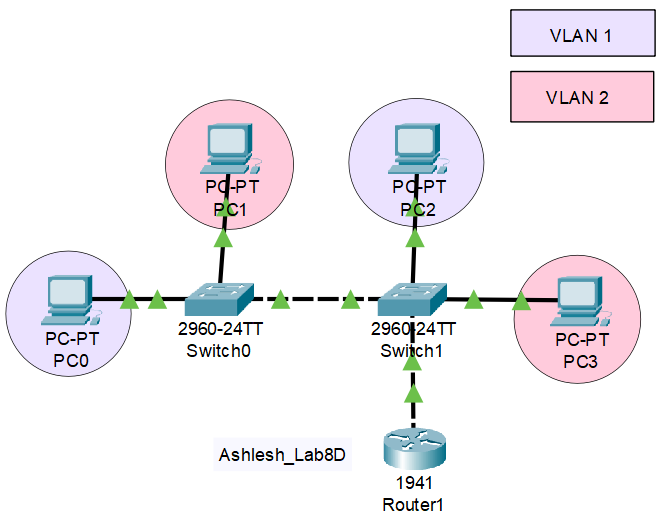
\includegraphics[scale=.9]{Figures/activityd.png}
	\caption{Simulated network for Activity D}
	\label{fig:activityd}
\end{figure}

\section{Exercises}
\problem{What is VLAN? Explain its importance in networking.}
VLAN, abbreviation to Virtual Local Area Network is a logical grouping of devices in the same broadcast domain regardless of their physical layout. VLANs have their own broadcast domain and subnets which allows segmented broadcast domains in layer 2 devices as well.  VLANs allow devices on physically different locations to exist in a single simulated virtual environment as if they were in the same LAN. This ensures proper network management, scalability and adaptability. VLANs can be used to divide a single ethernet switch as if it were multiple switches with each interface being assigned a separate VLAN. Additional importance of VLAN configuration in networking are listed as,
\begin{itemize}
    \item Additional security segregation can be opted by the administrator where sensitive hosts can be placed in an isolated VLAN.
    \item VLANs decrease the broadcast domain size without the increase in number of routers, which in turn limits traffic.
    \item It decreases network latency since number of hops are reduced significantly.
    \item Relocation of a device on the network is made easier.
\end{itemize}
\problem{How VLAN can be configured? Explain each step in detail.}
The configuration of VLAN follows the following steps,
\subsubsection*{1. Creating VLANs in a switch}
This step deals with creating VLANs on a switch. One VLAN is created on the switch by default and all the interfaces on the switch are assigned to this VLAN. To create additional VLANs on the switch, the following syntaxes are followed,
\syntax{config}{creating VLANs}
\subsubsection*{2. Assigning an interface to a VLAN}
This step deals with assigning interfaces to existing VLANs on the switch. By default all interfaces are assigned to VLAN 1, but they can be reassigned to a different VLAN as,
\syntax{assign}{assigning an interface to a particular VLAN}
\subsubsection*{3. Trunk port configuration}
This step deals with an interface on the switch being configured as a trunk port, which a link that carries multiple signals simultaneously to provide network access between two points. A trunk port is by default the member of all existing VLANs on the switch. It is used to connect two switches that have VLANs configured in them so that proper connection is estabilished between the two switches. 
\syntax{trunk}{configuring an interface as trunk port}
\syntax{manipulation}{manipulating VLANs in trunk port}
\problem{How packets can be forwarded between computers within same VLAN but connected at different switches? Explain.}
Computers in same VLAN but in different switches are disconnected due to the fact that they're in different swtiches and no link exists between them. A proper network connection between the two switches that have computers that are logically in the same VLAN can be estabilished in two ways,
\subsubsection*{1. Point-to-point connection between two interfaces on the same VLAN}
For two switches that have vlan\_1 and vlan\_2 configured on both of them, a connection between the two switches via interfaces that are assigned as vlan\_1 and vlan\_2 results in a connection between the devices that are on the same VLAN but on different switches. This way of establishing such a connection isn't optimal as the number of links goes on increasing with the increase in the number of VLANs that need to be connected.
\subsubsection*{2. Trunk port connection}
For two switches that have vlan\_1 and vlan\_2 configured on both of them, a connection between the two switches via interface that is assigned as trunk port with the two VLANs being allowed via trunk port results in a connection between the devices that are on same VLAN but on different switches. Trunking includes the VLAN information of all the VLANs that are allowed via trunk ports in the single link. The destination deframes this information and forwards the respective packet to the correct VLAN. This way of establishing a connection between devices on the same VLAN but on different switches is the optimal approach since only one trunk port is enough to carry the information and packets of the different VLANs on the switches.
\problem{How packets can be routed between computers at different VLANs? Explain.}
Computers in different VLANs are disconnected due to the fact that they are in logically different LANs. A proper network connection between the computers in different VLANs can be established in two ways,
\subsubsection*{1. Using a third switch with a single VLAN}
For two VLANs vlan\_1 and vlan\_2, a connection between the ports that are assigned as vlan\_1 and vlan\_2 and ports on a second switch that has only one VLAN results in connection between the two VLANs. This is only suitable if the two VLANs that need to be connected fall under the same subnet of the network. Such a connection can be regarded as a basic connection of two smaller segments of LANs into a single switch.
\subsubsection*{2. Inter-VLAN routing}
This method of connecting two different VLANs isn't dependent on the subnets that the VLANs fall under since it makes use of a router to route the packets to and from the VLANs. This method can be subdivided into two ways of connections as,
\subsubsection*{a. Point-to-point connection between interfaces on router and VLANs}
For two VLANs, vlan\_1 and vlan\_2, a connection between two interfaces that are assigned as vlan\_1 and vla\_2 with two interfaces of the router such that default gateway for all devices on the respective VLANs is set to the IP address of the interface connected to those VLANs results in a connection between the two VLANs regardless of the subnet they are in. This can be considered as two switches being connected to a router with proper default gateways being set. This way of inter-VLAN routing isn't feasible as the number of VLANs increases since multiple ports won't be available on the router for connection. 
\subsubsection*{b. Router on a stick}
An optimal approach to establish connection between two different VLANs is the router on a stick. For two VLANs, vlan\_1 and vlan\_2, a connection between sub-interfaces on the routers with proper encapsulation tags and a trunk port with the two VLANs being allowed via the trunk port added with default gateway for all devices on the respective VLANs being set to the IP address of the sub-interfaces being assigned to those VLANs results in a connection between the two VLANs. Inter-VLAN routing is acheived using the following syntax,
\syntax{inter}{configuration of router on a stick}
\problem{Note down the results of each step of the lab exercises and also explain with reason.}
\pagebreak
\subproblem{Activity A}
\addtocontents{lol}{\protect\subsection*{Activity A}}
\addtocontents{lot}{\protect\subsection*{Activity A}}

\subsubsection*{Sub activity 1}
\addtocontents{lot}{\protect\subsubsection*{Sub activity 1}}

\begin{table}[H]
	\centering
	\begin{threeparttable}
		\setting{Device}{
			PC0 & 200.1.1.2  & 255.255.255.0 \\
			PC1 & 200.1.1.66  & 255.255.255.0 \\
			PC2 & 200.1.1.3  & 255.255.255.0 \\
			PC3 & 200.1.1.67  & 255.255.255.0 \\
		}
		\begin{tablenotes}
			\small
			\item Note: The ip addressess and subnet masks are set using the IP configuration application.
		\end{tablenotes}
		\caption{IP address and subnet masks for the PCs and servers in the network}
		\label{tbl:pcsettinga}
	\end{threeparttable}
\end{table}

\subsubsection*{Sub activity 2}
\addtocontents{lol}{\protect\subsubsection*{Sub activity 2}}
\pingtest{a2}
By default all the interfaces on a switch are under the same VLAN, vlan 1. Since all the PCs fall under the same subnet for the mask 255.255.255.0, and the interfaces they are connected to are in the same VLAN, the ping tests frpm each PC to the other succeeds.

\subsubsection*{Sub activity 3}
\addtocontents{lol}{\protect\subsubsection*{Sub activity 3}}
\customcaption{a3}{Syntax for creating VLAN 2 on both switches}

\subsubsection*{Sub activity 4}
\addtocontents{lol}{\protect\subsubsection*{Sub activity 4}}
\customcaption{a4}{Syntax for assigning given interfaces to VLAN 2}

\subsubsection*{Sub activity 5}
\addtocontents{lol}{\protect\subsubsection*{Sub activity 5}}
\pingtest{a5}

\subsubsection*{Sub activity 6}
No, the ping test from PC1 to PC3 doesn't succeed. Although the two PCs under consideration are in the same VLAN and the same subnet, there is no connection between the two which results in a failed ping test. Similar pair of PCs, viz. PC0 and PC2 results in a successful ping test due to the connection of fastethernet0/10 of switch0 and fastethernet0/10 of switch1. 

\subsubsection*{Sub activity 7}
To solve the issue mentioned in sub activity 6 above, a connection between interface fastethernet0/12 of switch0 and fastethernet0/12 of switch1 is made. 

\subsubsection*{Sub activity 8}
\addtocontents{lol}{\protect\subsubsection*{Sub activity 8}}
\pingtest{a8}

\subsubsection*{Sub activity 9}
Yes, the ping test from PC1 to PC3 succeeds. The connection made in sub activity 7 makes sure that the two switches that have the PCs under the same VLAN have a proper connection. This is equivalent to two switches being connected with PCs in the same VLAN which is why the ping succeeds. 

\subsubsection*{Sub activity 10}
No, the ping test from PC0 to PC1 doesn't succeed. Although the two PCs under consideration are in the same subnet and even connected in the same switch, the ping test fails due to the fact that the two PCs are in different VLANs. This is equivalent to the PCs being connected in two different switches without a proper connection between the two which is why the ping fails.

\subsubsection*{Sub activity 11}
To solve the issue mentioned in sub activity 10 above, connection of fastethernet0/9 of switch1 with fastethernet0/9 of switch2 and
fastethernet0/13 of switch1 with fastethernet0/13 of switch2 is made.

\subsubsection*{Sub activity 12}
\addtocontents{lol}{\protect\subsubsection*{Sub activity 12}}
\pingtest{a12}

\subsubsection*{Sub activity 13}
Yes, the ping test from PC0 to PC1 succeeds. The connection made in sub activity 11 makes sure that the two VLANs are connected to a third switch with only one VLAN hence completing the connection. It is to be noted that the PCs are in the same subnet which is why the ping test succeeds upon proper connection.

\subproblem{Activity B}             
\addtocontents{lol}{\protect\subsection*{Activity B}}

\subsubsection*{Sub activity 1}
\addtocontents{lol}{\protect\subsubsection*{Sub activity 1}}
\customcaption{b1}{Syntax for configuring given interfaces as trunk port}
Listing~\ref{lst:b1} provides the syntax for configuring the given interface fastethernet0/20 on both switch0 and switch1. The interfaces are then used to connect the two switches rather than individual connections for each VLAN.

\subsubsection*{Sub activity 2}
\addtocontents{lol}{\protect\subsubsection*{Sub activity 2}}
\pingtest{b2}

\subsubsection*{Sub activity 3}
No, the ping test from PC0 to PC1 doesn't succeed. Although the two PCs under consideration are in the same subnet and even connected in the same switch, the ping test fails due to the fact that the two PCs are in different VLANs.
\subsubsection*{Sub activity 4}
Yes, the ping test from PC0 to PC2 succeeds. The connection made in sub activity 1 makes sure that the two switches that have the PCs under the same VLAN have a proper connection via the trunk port.
\subsubsection*{Sub activity 5}
Yes, the ping test from PC1 to PC3 succeeds. The connection made in sub activity 1 makes sure that the two switches that have the PCs under the same VLAN have a proper connection via the trunk port.
\subsubsection*{Sub activity 6}
\addtocontents{lol}{\protect\subsubsection*{Sub activity 6}}
To interconnect the two VLANs, connection of fastethernet0/9 of switch1 with fastethernet0/9 of switch2 and fastethernet0/13 of switch1 with fastethernet0/13 of switch2 is made.
\pingtest{b6}
All the ping tests succeeds. The connection made in sub activity 6 makes sure that the two VLANs are connected to a third switch with only one VLAN hence completing the connection. It is to be noted that the PCs are in the same subnet which is why the ping test succeeds upon proper connection.
\subsubsection*{Sub activity 7}
The configuration at the end of activity A and activity B are quite similar expect for a key difference in the way the two switches, switch0 and switch1 are connected. In the prior activity, the swtiches were connected using two interfaces, viz. fastethernet0/10 and fastethernet0/12 belonging to vlan 1 and vlan 2 respectively. The configuration at the end of activity B has a connection between the two switches via the fastethernet0/20 interfaces which has been configured as the trunk port in both the switches. This link is enough to carry the packets as well as vlan information between the switches which is then utilized by the receiving end to properly identify the vlan the packet is for. This shows the utility of a trunk port since it can drastically reduce the number of connections needed between two switches. 

\subproblem{Activity C}
\addtocontents{lol}{\protect\subsection*{Activity C}}
\addtocontents{lot}{\protect\subsection*{Activity C}}

\begin{table}[H]
	\centering
	\begin{threeparttable}
		\setting{Device}{
			PC0 & 200.1.1.2  & 255.255.255.192 \\
			PC1 & 200.1.1.66  & 255.255.255.192  \\
			PC2 & 200.1.1.3  & 255.255.255.192  \\
			PC3 & 200.1.1.67  & 255.255.255.192  \\
		}
		\begin{tablenotes}
			\small
			\item Note: The ip addressess and subnet masks are set using the IP configuration application. The default gateway of PC0 and PC2 is set as 200.1.1.1 and that of PC1 and PC3 as 200.1.1.65.
		\end{tablenotes}
		\caption{IP address and subnet masks for the PCs and servers in the network}
		\label{tbl:pcsettingc}
	\end{threeparttable}
\end{table}

\subsubsection*{Sub activity 1}
\addtocontents{lol}{\protect\subsubsection*{Sub activity 1}}
\pingtest{c1}
\subsubsection*{Sub activity 2}
The default gateway for all the PCs are set according to the Table~\ref{tbl:pcsettingc}.
\subsubsection*{Sub activity 3}
The switch2 is replaced by a router as instructed.
\subsubsection*{Sub activity 4}
\addtocontents{lot}{\protect\subsubsection*{Sub activity 4}}
\begin{table}[H]
	\centering
	\begin{threeparttable}
		\setting{Interfaces}{
			Router 0: 0/0 & 200.1.1.1  & 255.255.255.192 \\
			Router 0: 0/1 & 200.1.1.65  & 255.255.255.192 \\
		}
		\begin{tablenotes}
			\small
			\item Note: The interfaces are connected as, fastethernet0/8 of switch1 to gigabitethernet0/0 of router0 and fastethernet0/14 of switch1 to gigabitethernet0/1 of router0.
		\end{tablenotes}
		\caption{IP address and subnet masks for the gigabitethernet interfaces on the router}
		\label{tbl:gigasettingc}
	\end{threeparttable}
\end{table}
\subsubsection*{Sub activity 5}
\addtocontents{lol}{\protect\subsubsection*{Sub activity 5}}
\pingtest{c5}
Yes, the ping test succeeds in all cases. Although there are PCs that are in different VLANs and in different subnets, the router along with properly set default gateway makes sure that the data packets are properly routed to the correct VLAN destination. The trunk port connection between the two switches allows the PCs in the same VLAN to be connected. The overall configuration is equivalent to two switches being connected to the router with the proper gateways being set, which is why the ping succeeds.

\subproblem{Activity D}
\addtocontents{lol}{\protect\subsection*{Activity D}}
The connections between switch1 and router0 are removed and the IP address of the interfaces on the router are reset. 
\subsubsection*{Sub activity 1}
\addtocontents{lol}{\protect\subsubsection*{Sub activity 1}}
\customcaption{d1}{Syntax for configuring given interface as trunk port}
The trunk port, i.e. fastethernet0/21 on the swtich1 is connected to the gigabitethernet0/0 interface on the router.
\subsubsection*{Sub activity 2}
\addtocontents{lol}{\protect\subsubsection*{Sub activity 2}}
\customcaption{d2}{Syntax for configuring sub-interfaces on the router to work with the trunk port connection}
\subsubsection*{Sub activity 3}
\addtocontents{lol}{\protect\subsubsection*{Sub activity 3}}
\pingtest{d3}
Yes, the ping test succeeds in all cases. Although there are PCs that are in different VLANs and in different subnets, the router along with properly set default gateway as the equivalent sub-interface encapsulation as shown in Listing~\ref{lst:d2} make sure that the packets are properly forwarded to the correct VLAN. The interconnection of same VLANs on the different switches is made possible by the trunk port connecting switch0 and switch1, whereas the inter VLAN routing is acheived by router on a stick configuration with the trunk port fastethernet0/21 of swtich1 being connected with the gigabitethernet0/0 of the router. The interface is sub-divided into sub-interfaces that are given individual IP addressess and subnet masks giving a fully connected network. 
\subsubsection*{Sub activity 4}
The configuration at the end of activity C and activity D have a key difference in the way the switch1 and router0 are connected. In the prior activity, the devices were connected using two interfaces, viz. fastethernet0/10 and fastethernet0/12 belonging to vlan 1 and vlan 2 respectively on the switch with the gigabitethernet0/0 and gigabitethernet0/1 on the router. The configuration at the end of activity D has a connection between the switch and the router via the fastethernet0/21 interface which has been configured as the trunk port. This link is enough to carry the packets as well as vlan information between the switch and the router which is then deframed by the router based on the encapsulation performed on the router. This shows the utility of a trunk port with a router-on-a-stick configuration. This is one of the most frequently used configurations for the utlization of VLAN in network topologies.

\section{Conclusion}
The activities provided in the lab sheet were performed in the given order that allowed us to understand the concepts of VLAN configuration, forwarding and routing packets in VLANs. While performing activity A, the basics of configuring VLAN in switches was dealt. There were cases where PCs on the same subnet and even connected on the same switch would behave as though they weren't connected, which was a prime example of VLAN configuration. The concepts of VLAN separation allowed us to come up with a connection between the VLANs such that the ping tests would succeed. This was acheived with an additonal switch which acted as a means to connect the two logically isolated blocks since the additonal switch had only one VLAN by default. Moreover, on performing activity B, the concepts of trunk ports were understood. During activity A, the number of connection required to connect the switches would increase with the increase in same VLANs on the two switches. This wouldn't be a feasible approach to VLAN packet forwarding, which is why we assigned trunk ports on both the routers and used them to connect the swtiches such that all the VLANs were allowed in the trunk port giving us the equivalent connection. The configuration on the PCs upto this point made sure that they were in the same subnet, so only a proper connection would be enough to forward the packets. But in activity C, once the subnet mask of the PCs was changed, there were instances where some PCs were in different subnets than the other. To overcome the routing problems introduced, we replaced the additional switch with a router. With the default gateway for the devices on the respective VLANs being set to the IP addresses of the interfaces that they were connected to ensured that the ping tests succeed. Although we had a properly connected network, this method of inter VLAN routing isn't optimal. As the number of VLANs increases, individual connections are needed on the router, which isn't feasible. To overcome this flaw, router-on-a-stick approach was opted in acitivity D. To configure router-on-a-stick, one of the ports on the switch1 was assigned as a trunk port. This trunk port was then connected to one of the interfaces on the router. Furthermore, the interface was subdivided into subinterfaces that had the proper IP addresses and subnet masks as the two subnets, which were also used as the default gateway by the devices on the two VLANs. The complete network was fully connected with two VLANs being routed by the router using a router-on-a-stick configuration. The completion of this lab experiment allowed us to learn about the configuration of VLANs, it's practical implementations, trunk ports to forward packets and different ways of routing packets in a VLAN setup.
\end{document}